\chapter{Umsetzung Teilprojekt ITS}
\section{Netzwerkinfrastruktur Stand}
\subsection{Netzwerkaufbau}
Zunächst wurde das Projekt mit dem Router 4331 und mit einem zusätzlichen Modul (NIM-ES2-4) gestartet, um den Router um 4 weitere Gigabit Ports erweitert, da jeweils ein AP einen Port belegt, der Radius Server einen Port belegt, und ein Port mit „dem Internet“ verbunden ist. Standardmäßig ist der Router allerdings nur mit zwei Gigabit Ports bestückt. Einen weiteren könnte man mit dem GLC-T Modul erweitern, dann wäre man aber nur bei 3 statt 4 Ports. Der Port, der „mit dem Internet“ verbunden ist, erhielt zusätzlich ein GLC-GE-100FX Modul, da man darüber über 2km Reichweite mit Glasfaser erreichen könnte, und das am ehesten der Realität entspricht. 
Dass mehr Ports benötigt werden, ist erst beim Aufbauen des Netzwerkes aufgefallen. Daher musste der Router einmal ausgeschaltet werden und mit den Modulen erweitert werden. Dabei hat sich der Befehl „wr“ bzw. „write memory“ als sehr wichtig herausgestellt, da andernfalls alle bisherigen Konfigurationen gelöscht werden, da sie flüchtig waren.
Nachdem fast alle verkabelt war, außer der Radius Server, hat sich allerdings herausgestellt, dass das NIM-ES2-4 Modul nur auf Layer 2 arbeitet, also wie ein Switch. Es fehlte also ein Port für den Radius Server. Daher wurde der Router verworfen und es wurde ein PT-Empty mit 3x PT-ROUTER-NM-1CGE Modulen und einem PT-ROUTER-NM-1FGE Modul erweitert. Erstere werden verwendet, da die verwendeten AP nicht mit FastEthernet gearbeitet haben, und Letztere, um hohen Datentransfer zum Server zu gewährleisten. Vorteil: Der Router ist insgesamt günstiger als der ISR 4331, und er ist flexibel erweiterbar. Für diese Migration wurden die Konfigurations-Dateien der bisherigen Router exportiert, und in die neuen Router gemerged. Damit mussten die dhcp Konfigurationen nicht neu erstellt werden.
Nachdem das Netzwerk soweit eingerichtet wurde, und es an die Konfiguration des RADIUS-Servers ging, hat sich herausgestellt, dass die im Vergleich zu den LWAPs günstigeren APs nicht direkt einen RADIUS-Server angeben können. Daher wurde ein PT-ROUTER-NM-1CGE und der RADIUS-Server als solcher entfernt, dass die Kosten abermals reduziert. Das fertige Projekt lässt sich Preis-Leistungstechnisch kaum weiter optimieren, da man trotz der geringen Gesamtkosten immer noch ein hohes Maß an sowohl Geschwindigkeit als auch Sicherheit erreicht. Näheres dazu unter dem Reiter WLAN, Zugang und Sicherheit. 
Im Folgenden die Tabelle für die Subnetze und die Netzwerkskizzen für das Messe-Netzwerk und das Netzwerk in der Firmenzentrale:

\begin{table}[h]
	\centering
	\begin{tabular}{p{0.2\linewidth}|p{0.2\linewidth}|p{0.6\linewidth}}
		Netzwerk-Adresse & Subnetzmaske & Beschreibung \\ \hline
		192.168.4.128 & 255.255.255.224 & Dieses Netzwerk ist für die Firmengeräte auf der Messe gedacht. Es hat einen CIDR von /27, sodass alle 16 Geräte + Netzwerkadresse + Broadcastadresse in das Netz passen \\ \hline
		192.168.4.161 & 255.255.255.248 & Dieses Netzwerk ist für die Kunden-Geräte auf der Messe gedacht. Es hat einen CIDR von /29, sodass alle 4 Geräte + Netzwerkadresse + Broadcastadresse in das Netz passen \\ \hline
		142.250.183.0 & 255.255.255.0 & Dieses Netzwerk dient der Kommunikation zwischen dem Messe Router und dem Router der Firmenzentrale. Sie ist willkürlich gewählt, da sie normalerweise vom ISP vergeben wird, da das gleichzeitig auch die öffentliche IP-Adresse ist \\ \hline
		172.16.0.0 & 255.255.255.0 & Dieses Netzwerk soll das private Netzwerk innerhalb der Firmenzentrale darstellen. Da dieses nicht näher beschrieben wurde, wurde auch dieses willkürlich gewählt 
	\end{tabular}
\caption{Netzwerke für das Subnetting}
\end{table}

\begin{figure}[h]
	\centering
	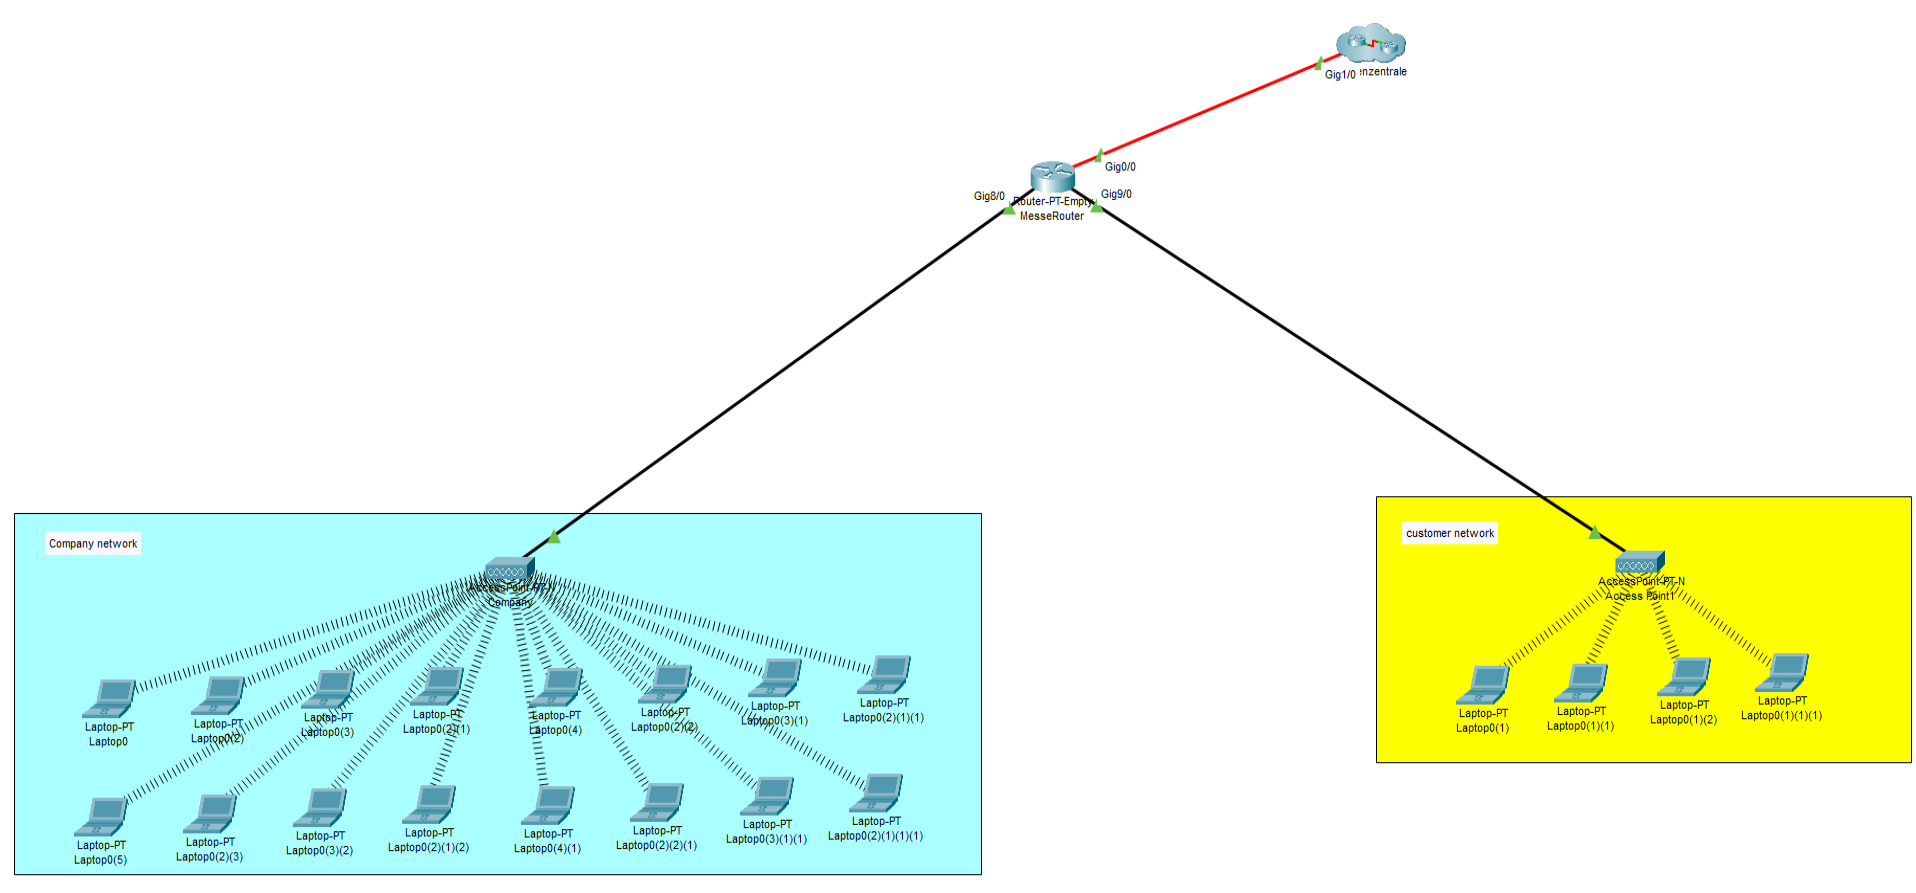
\includegraphics[width=0.95\linewidth]{Images/Netzwerk1}
	\caption{Netzwerkskizze Messe-Netzwerk}
	\label{fig:netzwerk1}
\end{figure}

\begin{figure}[h]
	\centering
	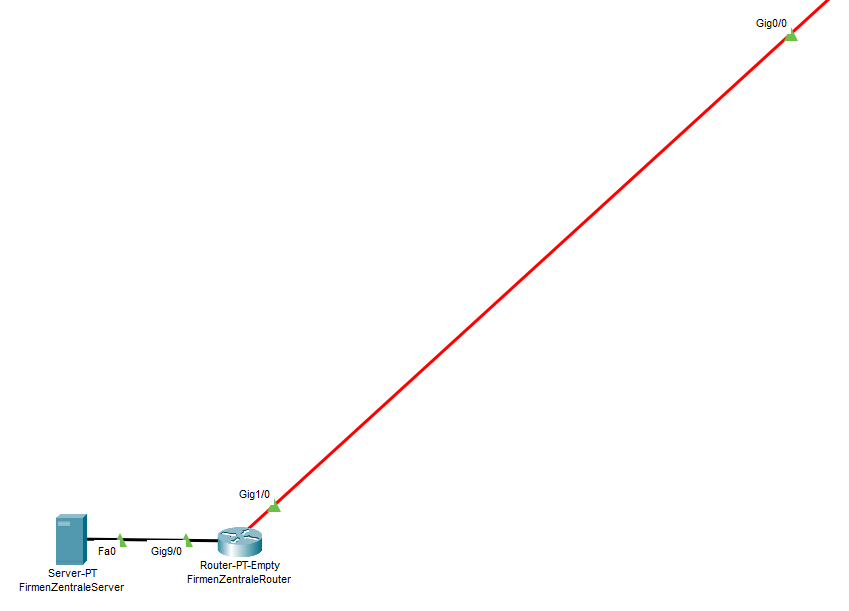
\includegraphics[width=0.7\linewidth]{Images/Netzwerk2}
	\caption{Netzwerkskizze Firmenzentrale-Netzwerk}
	\label{fig:netzwerk2}
\end{figure}

\newpage

\subsection{Anbindung Messenetzwerk}
\subsubsection{Messe Router Interface Konfiguration}
Das linke, untere Interface gig 8/0 befindet sich im company network, es ist also das größere Subnetz, da 16 Geräte benötigt werden. Die IP-Adresse lautet: 192.168.4.129 /27 (255.255.255.224). Die Subnetzmaske /28 konnte nicht verwendet werden, da neben den 16 Hosts auch eine Adresse für das Netzwerk und eine als Broadcastadresse verwendet wird.
Das rechte, untere Interface gig 9/0 befindet sich im customers network für die Kunden-Geräte. Dessen IP-Adresse lautet: 192.168.4.161 /29 (255.255.255.248). Die nächstkleinere Subnetzmaske konnte aufgrund obiger Beschreibung ebenfalls nicht verwendet werden.
Das obere Interface gig 0/0, ist das Interface, das „ins Internet“ führt, und über das dann der Server in der Firmenzentrale erreicht werden soll. Seine IPv4 lautet: 142.250.183.14 /24 (generisch, da diese IP-Adresse normalerweise vom ISP bereitgestellt wird und es gemäß Aufgabenstellung keine weitere Einschränkung in Bezug auf diese Adresse gibt).

\subsubsection{Firmenzentrale Router Interface Konfiguration}
Der Port, der „aus dem Internet“ zugreifbar ist, ist Gig 1/0 zusammen mit einem PT-ROUTER-NM-1FGE Modul. Er hat die IPv4: 142.250.183.16 (generisch, da diese IP-Adresse normalerweise vom ISP bereitgestellt wird). Es wurde absichtlich eine Adresse innerhalb des gleichen Netzwerkes gewählt, da dies am ehesten der Simulation einer VPN-Verbindung entspricht. Aufgrund dieser Annahme, und da es sich nur um eine Simulation des Firmenservers handelt, wurde ansonsten keine weitere Konfiguration zum Beispiel in Form einer ACL angefertigt.
Der Port, der mit dem Server der Firmenzentrale verbunden ist, hat den Port Gig 9/0 und das Modul PT-ROUTER-NM-1CGE. Er hat die IPv4: 172.16.0.10 /24 (generische, private IP-Adresse mit generischer Subnetzmaske).


\subsection{Netzwerk Einrichtung und IP-Zuweisung}
Die interface Adressen wurden den ip dhcp excluded adressen hinzugefügt, auch wenn das beim int gig 0/0 nicht notwendig gewesen wäre, da er nicht in die dhcp pools eingreift. Default Router sind entsprechend die ip adressen der Schnittstellen des Routers für die dhcp pools, also 192.168.4.129 für den company dhcp pool und 192.168.4.161 für den customers dhcp pool. Der dhcp pool company ist wie oben beschrieben für die Firmengeräte gedacht und hat das Netzwerk 192.168.4.128 255.255.255.224. Der dhcp pool customers ist für die Kunden-Geräte gedacht und hat das Netzwerk 192.168.4.160 255.255.255.248.

\subsection{Routing}
Theoretisch hätte man auch OSPF auf den Routern konfigurieren können, da dies eher dem Szenario entspricht, dass man erst „über das Internet“ geht und dann auf den Firmen-Server zugreift, wenn es aber darum geht, dass man sich über einen VPN-Tunnel mit dem Firmen-Server verbindet, und die Laptops ausschließlich mit dem Firmen-Server kommunizieren sollen und sonst nichts anderes können sollen, dann entsprechen statische Routen eher dem Anwendungsfall, weswegen wir uns dafür entschieden haben. Aufgrund der statischen Routen, müssen sowohl für den Messe Router als auch für den Firmenzentrale Router Tabellen angefertigt werden.

\begin{table}[h]
	\centering
	\begin{tabular}{p{0.25\linewidth}|p{0.25\linewidth}|p{0.25\linewidth}|p{0.25\linewidth}}
		Ziel-Netzwerk & Ziel-Subnetzmaske & Next Hop & Quell-Port \\ \hline
		172.16.0.0 & 255.255.255.0 & 142.250.183.16 & Gig 0/0
	\end{tabular}
	\caption{Messe Router Routing Tabelle}
\end{table}

\begin{table}[h]
	\centering
	\begin{tabular}{p{0.25\linewidth}|p{0.25\linewidth}|p{0.25\linewidth}|p{0.25\linewidth}}
		Ziel-Netzwerk & Ziel-Subnetzmaske & Next Hop & Quell-Port \\ \hline
		192.168.4.128 & 255.255.255.224 & 142.250.183.14 & Gig 1/0 \\ \hline
		192.168.4.160 & 255.255.255.248 & 142.250.183.14 & Gig 1/0
	\end{tabular}
	\caption{Firmenzentrale Router Routing Tabelle}
\end{table}

\section{WLAN}
\subsection{Zugang und Sicherheit}
Der Zugriff auf das Netzwerk wurde mithilfe WPA2-PSK gesichert. Dieses Protokoll nutzt die AES-Verschlüsselung, die deutlich sicherer ist als TKIP, was noch von WPA verwendet wurde, und sich als Standard-Verschlüsselung etabliert hat. Da es sich nur um einen Messe-Aufenthalt handelt, muss man sich keine Gedanken über das zyklische tauschen des Schlüssels machen, was normalerweise der Fall wäre, um die Sicherheit zu erhöhen. Der Schlüssel wurde außerdem sehr lang gewählt, und wird in KeePass verschlüsselt gespeichert. Die Schlüssellänge wurde bewusst sehr lang gewählt, da es sowohl für die Firmengeräte als auch die Kundengeräte verwendet werden soll, was Administratoren die Arbeit erleichtert, da Sicherheit auch immer ein Abwägen zwischen Aufwand und Ertrag ist.
Wie im Kapitel „Routing“ bereits erwähnt, wird davon ausgegangen, dass nur über eine VPN-Verbindung der Firmenzentrale Server erreicht werden kann, was ein großes Plus an Sicherheit für die Kommunikation zwischen dem Messer Router und dem Firmenzentrale Netzwerk bedeuten würde. Diese Sicherheit, und die gesicherte Verbindung zwischen den APs wurde durch die beiden ACLs erreicht, die auf dem Messe Router konfiguriert wurden:

\subsubsection{ACL 1}
\subsubsection{Situationsbeschreibung}
Nur Requests vom Server an die Netzwerke sollen erlaubt werden. Die Kommunikation zwischen den Netzwerken und die Paket-Weiterleitung der Pakete an die Netzwerke von anderen IP-Adressen als der Server-Adresse sollen gestoppt werden. Für diesen Anwendungsfall reicht eine einfache ACL, da keine Protokolle spezifiziert werden müssen.

\subsubsection{Befehle}
\begin{itemize}
	\item access-list 1 permit 142.250.183.16 255.255.255.0
	\item (int 8/0) ip access-group 1 out $\rightarrow$ Das Paket darf nur von diesem Netzwerk in das Netzwerk kommen.
	\item (int 9/0) ip access-group 1 out
\end{itemize}

\subsubsection{ACL 101}
\subsubsection{Situationsbeschreibung}
Nur Anfragen an den Server aus den Netzwerken sollen erlaubt werden. Alle anderen Anfragen sollen fallen gelassen werden. Von den Anfragen, die zugelassen werden, sollen wiederum nur eine HTTPS Verbindung erlaubt werden, um zu gewährleisten, dass die Kommunikation verschlüsselt stattfindet. Dafür wird eine erweitere ACL benötigt, die TCP auf dem Standard-Port 443 erlaubt.

\subsubsection{Befehle}
\begin{itemize}
	\item access-list 101 permit tcp 192.168.4.129 0.0.0.31 172.16.0.10 0.0.0.255 eq 443
	\item access-list 101 permit tcp 192.168.4.161 0.0.0.7 172.16.0.10 0.0.0.255 eq 443
	\item (int gig 0/0) ip access-group 101 out
\end{itemize}

\subsubsection{Folgen}
Aufgrund dieser restriktiven Einstellung war es zeitweise nicht möglich, die Notebooks über dhcp zu konfigurieren, da die dhcp discovery packages gedroppt wurden.

\subsubsection{Lösung}
Daher müssen die UDP-Ports, die für DHCP verwendet werden, ebenfalls erlaubt werden, und da die Notebooks zu dem Zeitpunkt noch keine IP haben, und das interface nicht kennen, wird any any verwendet:
\begin{itemize}
	\item access-list 101 permit udp any any eq 67
	\item access-list 101 permit udp any any eq 68
\end{itemize}

\subsection{Anbindung von Clients}
Die Laptops haben standardmäßig ein Modul verbaut, welches nur einen Ethernet Port anbietet. Daher musste das integrierte Module der Laptops ausgebaut werden und durch ein WPC300N ersetzt werden, da dieses WLAN unterstützt. Um sich nun mit dem Netzwerk zu verbinden, muss man unter Desktop, PC Wireless, den nächsten AP auswählen und den Schlüssel eingeben. Ansonsten ist keine Verbindung mit dem Netzwerk möglich.

\section{Inbetriebnahme}
Bevor die Mitarbeiter auf die Messe fahren, sollten sie überprüfen, dass sie die 16 firmeninterne Laptops, die 2 APs, und den Router dabeihaben. Außerdem sollten sicherheitshalber LAN-Kabel mitgenommen werden, da wir nicht wissen, ob diese vor Ort verfügbar sind oder nicht. Da der Router und die firmeninternen Geräte vorkonfiguriert sind, müssen die Mitarbeiter die Komponenten nur noch an den Strom anschließen und starten. Vergewissern Sie sich, dass sie mit der Software vertraut sind und die Schulung verstanden haben. Bei Fragen zur Anwendung wenden Sie sich an die Mitarbeiter vor Ort. Es wird ein reibungsloser Ablauf erwartet, da es sonst rufschädigend sein könnte. Falls die Laptops den WLAN-Zugang nicht mehr gespeichert haben sollten, muss das WLAN mit der SSID company ausgewählt werden, und das folgende Passwort eingegeben werden:

JWB5EMkWFZeLtV1OVKaEqYhvxs3ICtw2

Die Kunden, von denen wir maximal 4 gleichzeitig bedienen können, nutzen das WLAN mit der SSID customers. Das Passwort hierfür ist jedoch das gleiche. Bitte stellen Sie sicher, dass sich die Kunden nach erfolgreicher Interaktion wieder von dem Netzwerk trennen, da sonst Plätze für neue Kunden blockiert werden würden.
 